\section{Introduction to Languages, IDE's, Tools and Technologies}

\subsection{Introduction to Languages}
Front End languages are language that are used to give better user experince and user interface. These mainly include HTML, CSS, JS. Some Frameworks like Bootstrap, Django are also used with these basic languages. Database used with this project is MySQL.
\subsubsection{HTML}

\begin{figure}[h]
\centering 
\includegraphics[scale=0.05]{input/images/HTML.png}
\caption{HTML5 logo}
\end{figure}
HyperText Markup Language, commonly referred to as HTML, is the standard markup language used to create web pages. Along with CSS, and HTML is a cornerstone technology, used by most websites to create visually engaging webpages, user interfaces for web applications, and user interfaces for many mobile applications. \\
Web browsers can read HTML files and render them into visible or audible web pages. HTML describes the structure of a website semantically along with cues for presentation, making it a markup language, rather than a programming language.\\
HTML elements form the building blocks of all websites. HTML allows images and objects to be embedded and can be used to create interactive forms. It provides a means to create structured documents by denoting structural semantics for text such as headings, paragraphs, lists, links, quotes and other items.

\begin{verbatim}
<!DOCTYPE html>
<html>
  <head>
    <title>This is a title</title>
  </head>
  <body>
    <p>Hello world!</p>
  </body>
</html>

\end{verbatim}


\subsubsection{CSS}

\begin{figure}[h!]
\centering 
\includegraphics[scale=0.50]{input/images/CSS.jpg}
\caption{CSS logo}
\end{figure}
Cascading Style Sheets (CSS) is a style sheet language used for describing the presentation of a document written in a markup language.Although most often used to set the visual style of web pages and user interfaces written in HTML and XHTML, the language can be applied to any XML document, including plain XML, SVG and XUL, and is applicable to rendering in speech, or on other media. \\
Along with HTML and JavaScript, CSS is a cornerstone technology used by most websites to create visually engaging webpages, user interfaces for web applications, and user interfaces for many mobile applications.\\
CSS is designed primarily to enable the separation of document content from document presentation, including aspects such as the layout, colors, and fonts.\\
 This separation can improve content accessibility, provide more flexibility and control in the specification of presentation characteristics, enable multiple HTML pages to share formatting by specifying the relevant CSS in a separate .css file, and reduce complexity and repetition in the structural content, such as semantically insignificant tables that were widely used to format pages before consistent CSS rendering was available in all major browsers.\\
 CSS makes it possible to separate presentation instructions from the HTML content in a separate file or style section of the HTML file. For each matching HTML element, it provides a list of formatting instructions

\begin{verbatim}
p {
    color: red;
    text-align: center;
} 
\end{verbatim}

\subsubsection{Javascript}
\begin{figure}[h]
\centering 
\includegraphics[scale=0.3]{input/images/JS.png}
\caption{Javascript logo}
\end{figure}
JavaScript is a high-level, dynamic, untyped, and interpreted programming language. It has been standardized in the ECMAScript language specification. Alongside HTML and CSS, it is one of the three essential technologies of World Wide Web content production; the majority of websites employ it and it is supported by all modern web browsers without plug-ins. JavaScript is prototype-based with first-class functions, making it a multi-paradigm language, supporting object-oriented, imperative, and functional programming styles. It has an API for working with text, arrays, dates and regular expressions, but does not include any I/O, such as networking, storage or graphics facilities, relying for these upon the host environment in which it is embedded.

\subsubsection{jQuery} 
\begin{figure}[h!]
\centering 
\includegraphics[scale=0.3]{input/images/jquery.png}
\caption{jQuery logo}
\end{figure}
jQuery is a cross-platform JavaScript library designed to simplify the client-side scripting of HTML. It is free, open-source software using the permissive MIT License. The purpose of jQuery is to make it much easier to use JavaScript on a website. jQuery takes a lot of common tasks that require many lines of JavaScript code to accomplish, and wraps them into methods that you can call with a single line of code.



\subsection{Introduction to Frameworks}
\subsubsection{Django}
\begin{figure}[h!]
\centering 
\includegraphics[scale=0.2]{input/images/django.png}
\caption{Djangologo}
\end{figure}
Django is a free and open-source web framework, written in Python, which follows the model-view-template architectural pattern. It is maintained by the Django Software Foundation, an independent organization. It is a high-level Python Web framework that encourages rapid development and clean, pragmatic design.


\subsubsection{Bootstrap}
\begin{figure}[h!]
\centering 
\includegraphics[scale=0.2]{input/images/boot.png}
\caption{BootStrap logo}
\end{figure}

Bootstrap is a free and open-source collection of tools for creating websites and web applications. It contains HTML and CSS-based design templates for typography, forms, buttons, navigation and other interface components, as well as optional JavaScript extensions. \\
It aims to ease the development of dynamic websites and web applications.\\
Bootstrap is a front end framework, that is, an interface for the user, unlike the server-side code which resides on the "back end" or server.

\subsection{Tools \& Technologies}

\subsubsection{Doxygen}
\begin{figure}[ht]
\centering 
\includegraphics[scale=1]{input/images/doxygen.jpeg}
\caption{Doxygen logo}
\end{figure}
\noindent Doxygen is a documentation generator, a tool for writing software reference 
documentation. The documentation is written within code, and is thus 
relatively easy to keep up to date. Doxygen can cross reference 
documentation and code, so that the reader of a document can easily 
refer to the actual code.
\begin{center}
\textbf{Features}
\end{center}
Doxygen is a tool to create a documentation for your program/project written in the languages like C, C++, Java, python and so on. It reads the well formatted and special doxygen comments to create the required documentation. This documentation is very important for the new developers who want to help in the development of the project. Documentation is one of the main pillar of an open-source project.
\begin{itemize}
\item Requires very little overhead from the writer of the documentation. 
Plain text will do, Markdown is support, and for more fancy or structured 
output HTML tags and/or some of doxygen's special commands can be used.
\item Cross platform: Works on Windows and many Unix flavors (including 
Linux and Mac OS X).
\item Comes with a GUI frontend (Doxywizard) to ease editing the options 
and run doxygen. The GUI is available on Windows, Linux, and Mac OS X.
\item Automatically generates class and collaboration diagrams in HTML 
(as clickable image maps) and $\mbox{\LaTeX}$ (as Encapsulated PostScript 
images).
\item Allows grouping of entities in modules and creating a hierarchy 
of modules.
\item Doxygen can generate a layout which you can use and edit to change 
the layout of each page.
\item Can cope with large projects easily.
\end{itemize}
\begin{center}
\textbf{Installation}
\end{center}
Doxygen can be installed using following commands:\\\\
\emph{
\$ git clone https://github.com/doxygen/doxygen.git\\\\
\$ cd doxygen\\\\
\$ ./configure\\\\
\$ make \\\\}
This will install Doxygen on your pc or laptop.\\
You can create the documentation using the graphical user interface (GUI) or console mode.\\\\
While writing the comments we have to follow a pattern with the tags i.e. before every tag we should have something special so that Doxygen can understand what are we creating. Actually Doxygen read these tags and place them at special location in the generated output. So, we have to specify them explicitly. 

\subsection{LaTeX}
\begin{figure}[!ht]
\centering
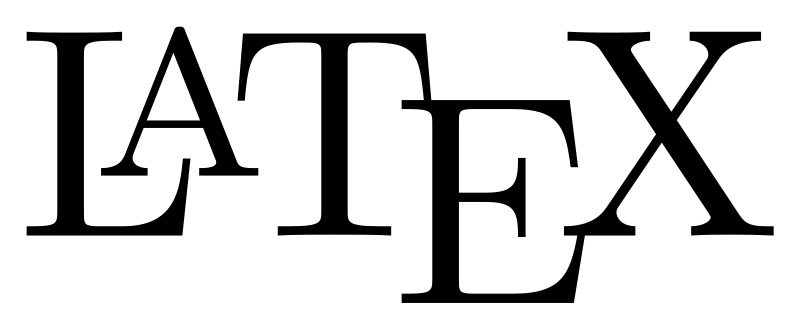
\includegraphics[width=0.3\textwidth]{input/images/latex.png}                   
\caption{\LaTeX} 
\hspace{-1.5em}
\end{figure}
\LaTeX is a document markup language and document preparation system for the \TeX{} 
typesetting program. Within the typesetting system, its name is styled 
as \LaTeX.

To run LATEX on your own computer, you need  to use a latex distribution. A distribution includes a latex program and (typically) several thousand packages.
\begin{itemize}
  \item  On Windows: MikTEX or TEXLive
   \item On Linux: TEXLive
  \item  On Mac: MacTEX
\end{itemize}
Apart from the pdf file; lat.aux, lat.log, lat.pdf files are created by default.\\
\begin{itemize}
\item AUX is a data file format used by Latex
AUX is a data file format used by LaTeX. LaTeX is a macro package which uses TeX typesetting language in its documents. AUX files contain information used for cross-referencing, and is also used to transport information from one compiler run to the next.
\item Some of the compilers are pdftex, Xelatex, Lualatex etc.
\item A log file is usually a flat text file that contains a list of events that happend when a program was running, with one event on each line. Often times errors are recorded in log files.
\item .pdf: The common output format for your document.
Created by pdflatex/ xelatex
\end{itemize}
\begin{figure}[!ht]
\centering
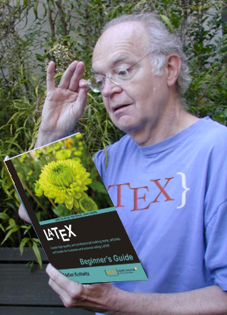
\includegraphics[width=0.3\textwidth]{input/images/donald.png}                   
\caption{Donald Knuth, Inventor Of \TeX{} 
typesetting system}
\hspace{-1.5em}
\end{figure}
\LaTeX was first developed in 1985 by Leslie Lamport.
In preparing a \LaTeX{} document, the author 
specifies the logical structure using familiar concepts such as 
chapter, section, table, figure, etc., and lets the \LaTeX{} system 
worry about the presentation of these structures. It therefore 
encourages the separation of layout from content while still allowing 
manual typesetting adjustments where needed. 

\subsubsection{MySQL} 
\begin{figure}[h!]
\centering 
\includegraphics[scale=0.2]{input/images/sql.png}
\caption{MySQL Database}
\end{figure}
MySQL is an open-source relational database management system. Its name is a combination of "My", the name of co-founder Michael Widenius's daughter, and "SQL", the abbreviation for Structured Query Language.\\
SQL is a standard language for storing, manipulating and retrieving data in databases.

\subsubsection{HoverCraft}
Hovercraft's power comes from the combination of reStructuredText's convenience with the cool of impress.js, together with a flexible and powerful solution to position the slides.\\
It creates wonderful presentations by providing an ease with the effects like Rotation, Zoom etc.




\subsubsection{Git \& GitHub}
\begin{figure}[!ht]
\centering

\includegraphics[width=0.3\textwidth]{input/images/github}                   
\caption{Github Logo}
\hspace{-1.5em}
\end{figure}
\leavevmode\\
GitHub is a Git repository web-based hosting service which offers all of the functionality of Git as well as adding many of its own features. Unlike Git which is strictly a command-line tool, Github provides a web-based graphical interface and desktop as well as mobile integration. It also provides access control and several collaboration features such as wikis, task management, and bug tracking and feature requests for every project.\\
\begin{center}\textbf{Installation}
\end{center}
Installation of git is a very easy process.
The current git version is: 2.0.4.
Type the commands in the terminal:\\\\
\emph{
\$ sudo apt-get update\\\\
\$ sudo apt-get install git\\\\}
This will install the git on your pc or laptop.

\begin{center}\textbf{Various Git Commands}
\end{center}
Git is the open source distributed version control system that facilitates GitHub activities on your laptop or desktop. The commonly used Git command line instructions are:-\\
For starting a new repository or obtaining from an exiting URL

\begin{description}

\item [\$ git init [ project-name]]\\
Creates a new local repository with the specified name
\item [\$ git clone [url]]\\
Downloads a project and its entire version history\\

\end{description}
\section{Project Scheduling}
The project schedule is the tool that communicates what work needs to be performed, which resources of the organization will perform the work and the timeframes in which that work needs to be performed. The project schedululing reflects all of the work associated with delivering the project on time.

\subsection{Gantt Chart}
A Gantt chart is a type of bar chart that illustrates a project schedule. This chart lists the tasks to be performed on the vertical axis, and time intervals on the horizontal axis.\\
A Gantt chart is a graphical depiction of a project schedule. A Gantt chart is a type of bar chart that shows the start and finish dates of several elements of a project that include resources, milestones, tasks and dependencies. \\\\

 \begin{figure}[!h]
	\centering 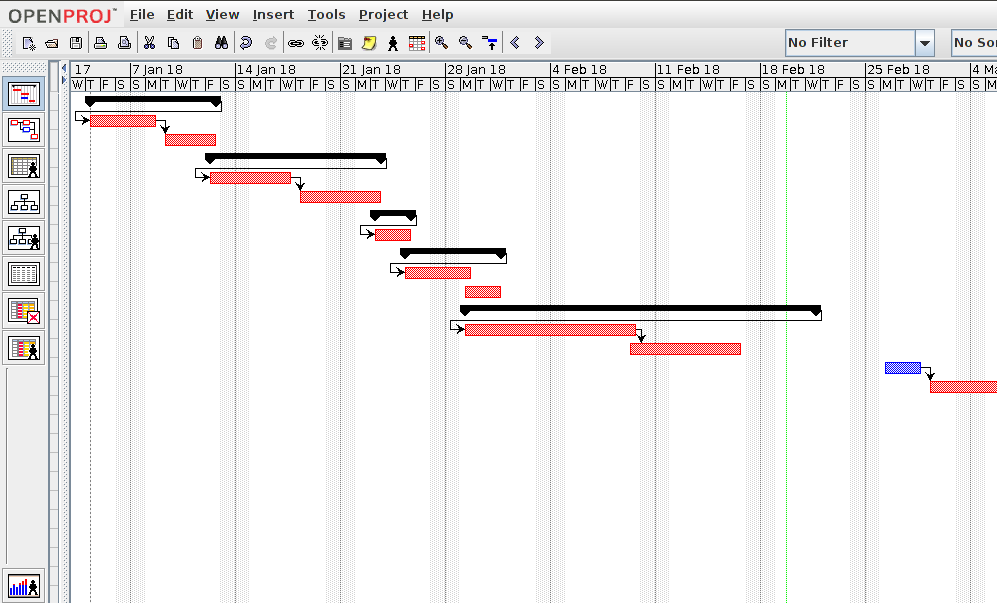
\includegraphics[scale=.43]{input/images/chart1.png}
	\caption{Gantt Chart}
\end{figure}

Gantt charts are most commonly used for tracking project schedules. For this it is useful to be able to show additional information about the various tasks or phases of the project, for example how the tasks \\
Gantt charts may be simple versions created on graph paper or more complex automated versions created using project management applications.
\newpage
\subsection{Network Diagram}
A Network Diagram is a visual representation of a project's schedule. A network diagram in project management is useful for planning and tracking the project from beginning to finish. It represents a project's critical path as well as the scope for the project.

 \begin{figure}[!h]
	\centering 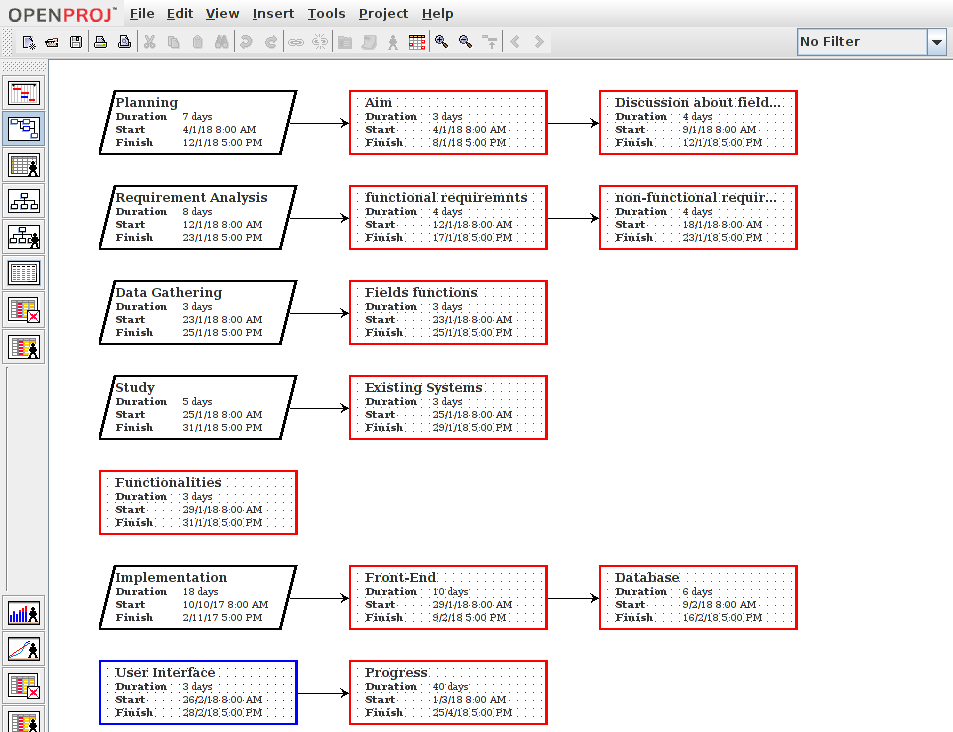
\includegraphics[scale=.43]{input/images/networkchart.png}
	\caption{Network Chart}
\end{figure}
\section{Testing}
Testing a program consists of providing the program with a set of test inputs (or test cases) and
observing if the program behaves as expected. If the program fails to behave as expected, then the
conditions under which failure occurs are noted for later debugging and correction. \\
This software had been taken through rigorous test to fully found potential causes of error and system failure
and full focus have been given to cover all possible exceptions that can 
occur and cause failure of the software.\\
As this software is based on intensive background process it have been taken care that 
if correct input and email address are given then processing of user job can even continue or a least automatically 
restart even after server shuts down or even crash.\\\\


\begin{table}[h]
\centering
\begin{tabular}{ ||c|c|| }
\hline
 \multicolumn{2}{||c||}{Overview of SamanyaSeva} \\
 \hline
 Module & Working \\ [0.5ex] 
 \hline \hline
 UserAccounts & Users Data \\ \hline
  Bills & Billing Module \\ \hline
  Catalog & A basic menu\\ \hline
  Reports & Maintained Registers \\ \hline
  Suspense & Payment \\ \hline
  Administration &  Admin Power \\ \hline
  
\end{tabular}
\caption{Modules}
\label{table2}
\end{table}

\begin{table}[h]
\centering
\begin{tabular}{ ||c|c|| }
\hline
 \multicolumn{2}{||c||}{Validations} \\
 \hline
 Validation & Error \\ [0.5ex] 
 \hline \hline
 Email & With the use of @ \\ \hline
GST Number & Alpha-Numeric Value \\ \hline
 Telephone & Numeric Only\\ \hline
 Date Format & Can't add in other formats \\ \hline
Mandatory Fields & Can't add data without defining Group name \\ \hline
 Admin Power &  Can't access Bills module without Admin rights \\ \hline
  
\end{tabular}
\caption{Validations}
\label{table2}
\end{table}







%\section{Software Requirements}
%\begin{itemize}
%	\item Apache Web Server
%	\item Python
%	\item Mysql server
%	\item Django
%	\end{itemize}



%\section{Hardware Requirements}
%\begin{itemize}
%\item Connectivity to the Internet
%\item Working System
%\item Operating System
%\item A server
%	\end{itemize}

%	\section{Expected Outcome}

%Professionally implemented CRM systems deliver many benefits for sales, marketing, service and other teams.
%The main purpose and expected result of SamanyaSeva is to support a business in engaging its customers.\\\\
%This application will also be developed using latest technologies and modular approach, so that anyone can further enhance this project by studying it's documentation and code.\\
%Aim is to enhance the operational efficiency of business resources and to assist organizations in achieving their goals at a faster rate and in an efficient manner.

